\section{Method}
\label{sec:method}

The pipeline runs the four stages of Fig.~\ref{fig:system-overview} in order, each consuming the output of the last.
The \emph{observe} stage collects $\mathcal{T}_\text{diag}$ at the deployment site.
The \emph{diagnose} stage maps $(\pi_\theta, \mathcal{T}_\text{diag})$ to per-region scores $D(r) \in (0, 1]$ through a comparison tier against a cached source reference and a reference-free tier, blended by a per-region Fr\'{e}chet gate (\S\ref{sec:method-diagnose}); the scores must agree with $\rho(r)$ in rank order within a deployment and in calibrated magnitude across deployments, since the allocator consumes both.
The \emph{allocate} stage maps the scores to the rank assignment $k(r)$ of Eq.~\ref{eq:budget-constraint}, proportional to $D(r)$ up to per-region cost and zero below a freezing threshold (\S\ref{sec:method-allocate}).
The \emph{adapt} stage trains LoRA adapters of the assigned ranks on $\mathcal{T}$ (\S\ref{sec:method-adapt}).
Each stage runs once per deployment, and only the adapt stage updates parameters.

%----------------------------------------------------------------------
\subsection{Network Region Partitioning}
\label{sec:method-regions}

Adaptation cost is measured, and adapters are attached, per region, so the partition determines both what the diagnostic can resolve and what the allocator can control.
We partition each VLA along its native module boundaries into the functional regions of Table~\ref{tab:region-partitions} rather than imposing a fixed schema, for three reasons.
Native boundaries coincide with changes in representational role, from modality-specific encoding through fusion to action decoding, so a shift confined to one modality maps onto few regions; they carry architecture-defined parameter counts, which fixes $c_1(r)$ without tuning; and they exist for every architecture, which makes the spectrum comparable across the five models without a learned or hand-designed partition per model.
Finer partitions raise diagnostic cost and make the per-region Fisher and gradient statistics noisier, and coarser ones merge regions with different roles, so the module level is the natural granularity.

\begin{table}[tbp]
    \centering
    \setlength{\abovecaptionskip}{0pt}
    \setlength{\belowcaptionskip}{2pt}
    \caption{Region partitions with approximate parameter counts. AR, Diff., and FM denote autoregressive, diffusion, and flow-matching decoding.}
    \label{tab:region-partitions}
    \scriptsize
    \renewcommand{\arraystretch}{0.92}
    \setlength{\tabcolsep}{3pt}
    \resizebox{\columnwidth}{!}{%
    \begin{tabular}{@{}lcl@{}}
        \toprule
        \textbf{Model (Params)} & \textbf{Dec.} & \textbf{Regions} \\
        \midrule
        OpenVLA-OFT (7B) & AR (par.) & DINOv2, SigLIP, Proj., LLaMA-e, LLaMA-l, Act.\ Head \\
        $\pi_0$ (3.3B)   & FM        & SigLIP, Gemma, Act.\ Expert \\
        SmolVLA (450M)   & FM        & SigLIP, SmolLM2, Proj., Act.\ Expert \\
        DTP (350M)       & Diff.     & DINOv2, CLIP, Q-Former, Diff.\ Trans. \\
        Octo (93M)       & Diff.     & Vis.\ Tok., T5 Enc., Transformer, Diff.\ Head \\
        \bottomrule
    \end{tabular}}
\end{table}


%----------------------------------------------------------------------
\subsection{Stages 1--2: Observe and the Two-Tier Diagnostic}
\label{sec:method-diagnose}

\begin{figure}[!tp]
    \centering
    \setlength{\abovecaptionskip}{4pt}
    \setlength{\belowcaptionskip}{-8pt}
    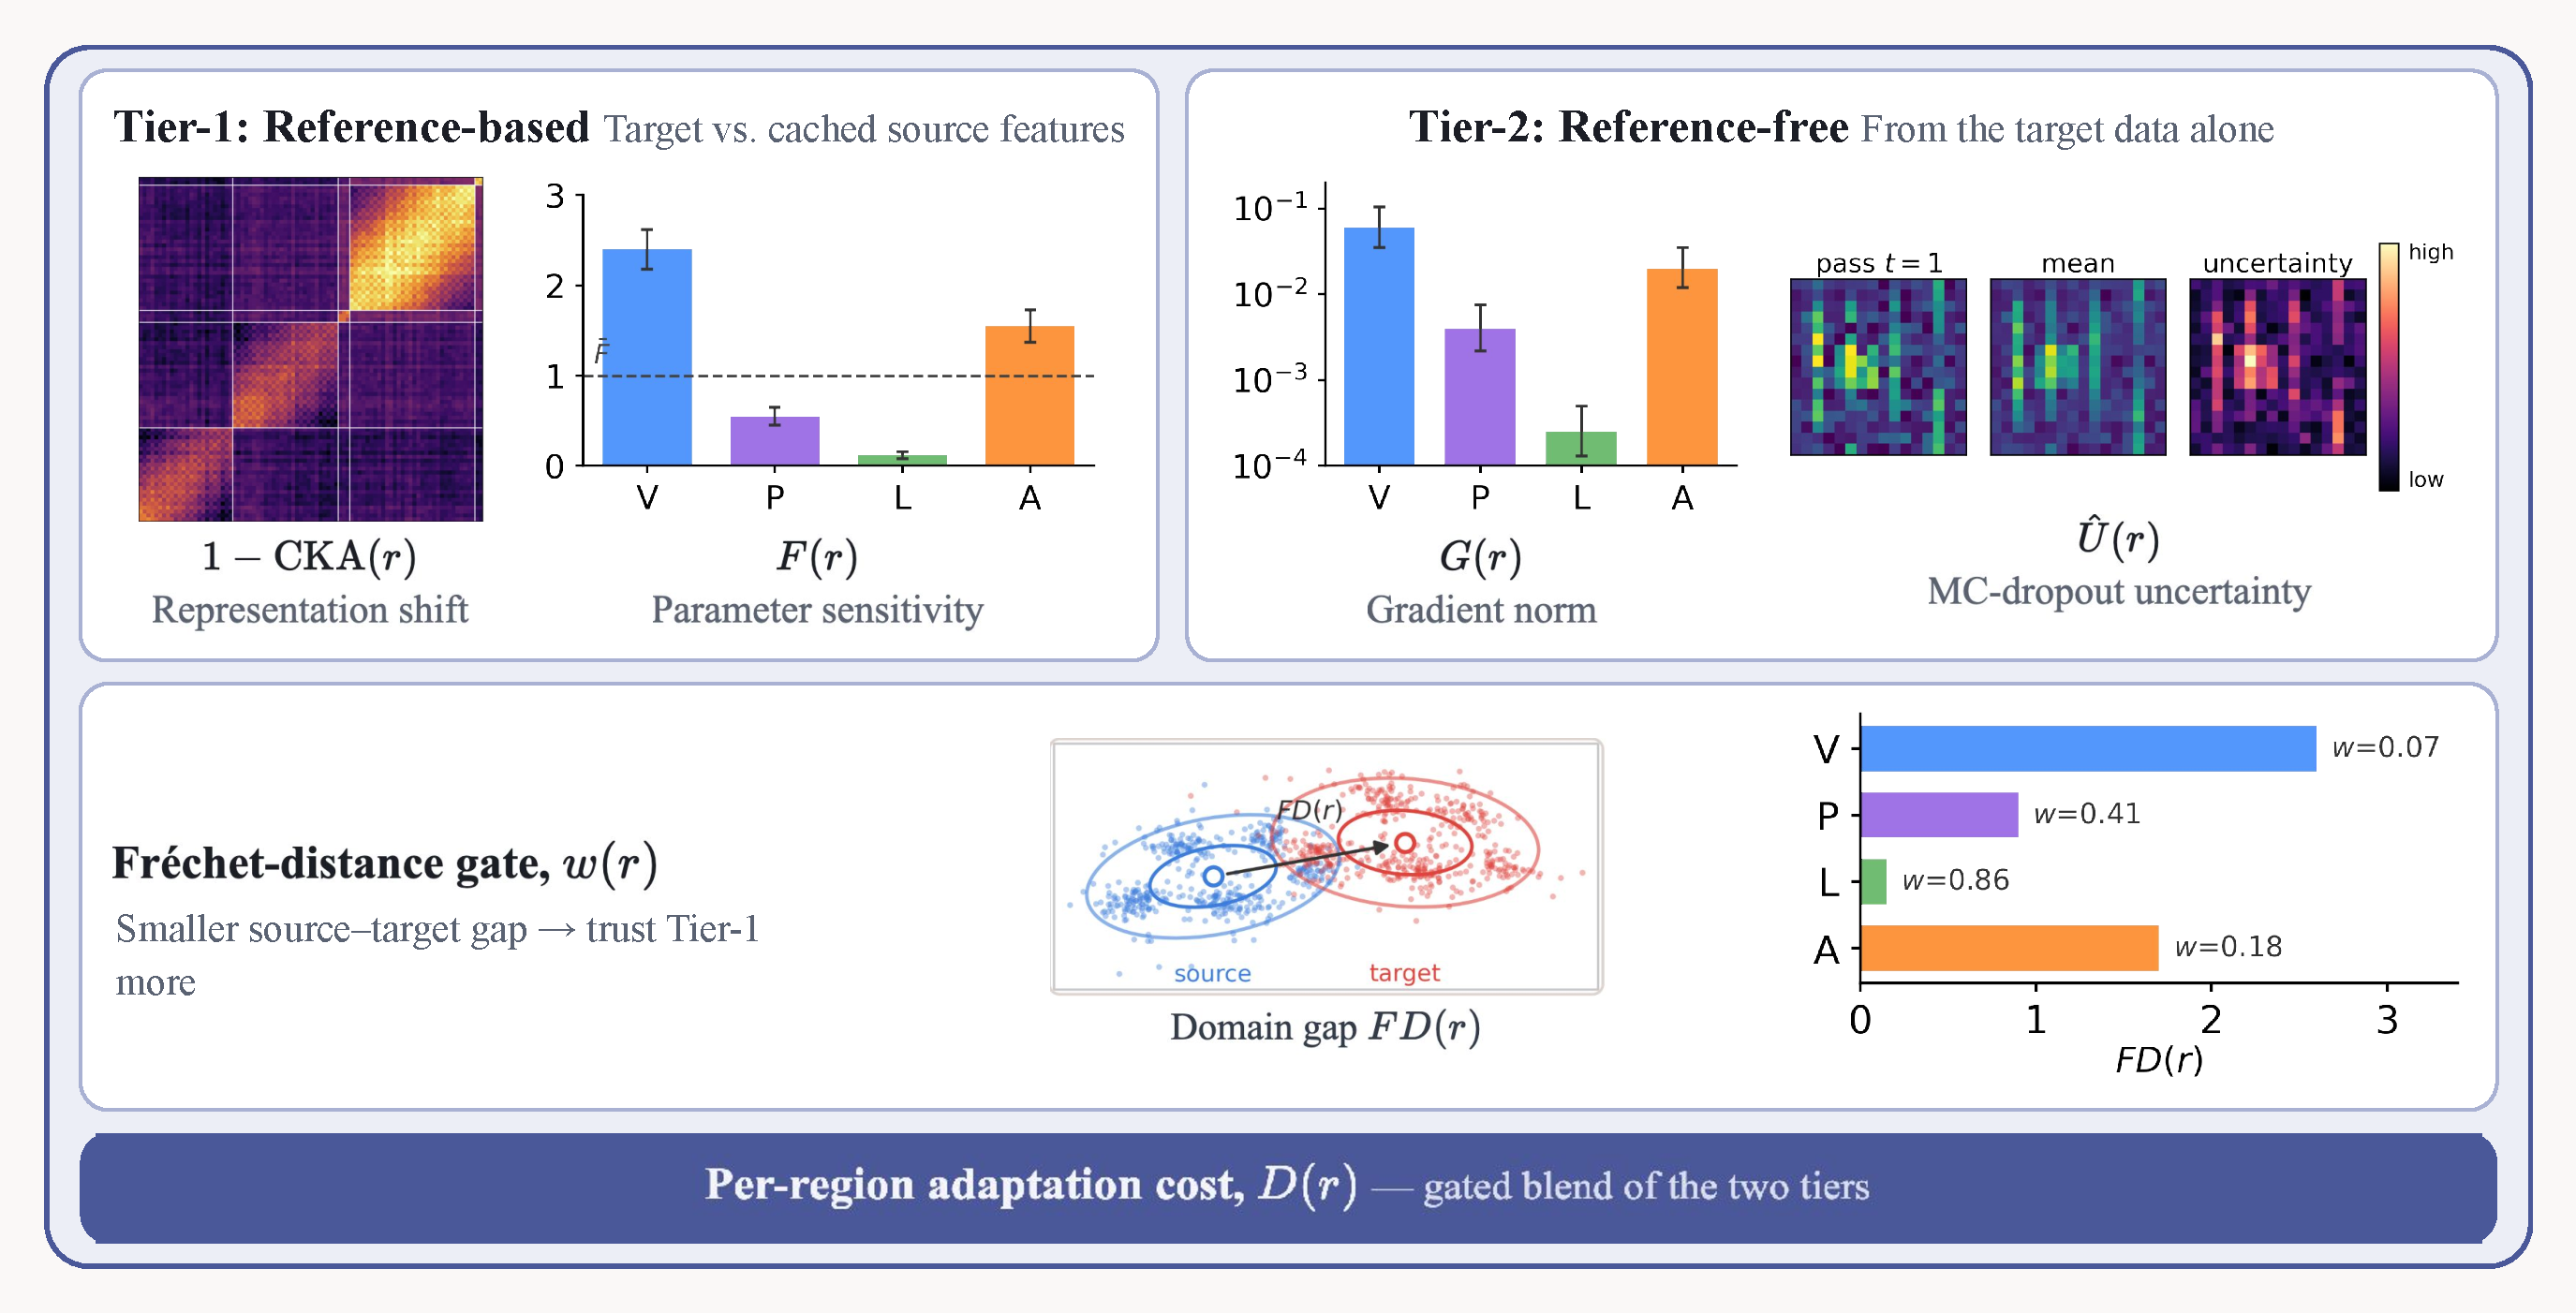
\includegraphics[width=\columnwidth]{images/diagnostic_figure.pdf}
    \caption{\textbf{The two-tier diagnostic.} Tier~1 scores representational shift ($1 - \mathrm{CKA}(r)$) against the cached source reference, weighted by Fisher sensitivity $\overline{F}(r)$ normalized to a global mean of one (dashed line); Tier~2 profiles the surrogate gradient norm $G(r)$ and MC Dropout uncertainty $\hat{U}(r)$ from target observations alone; the gate $w(r) = \exp(-\gamma \cdot \mathrm{FD}(r))$ trusts Tier~1 where the source--target gap is small, and the blend yields $D(r)$. V, P, L, and A denote vision encoder, projector, language backbone, and action head.}
    \label{fig:diagnostic}
\end{figure}

From the $N$ unlabeled observations $\mathcal{T}_\text{diag}$, the two-tier diagnostic estimates per-region cost with a small number of forward passes and one backward pass through the \emph{frozen} VLA, routing each region to the strongest available signal for its domain gap.

\paragraph{Cached source reference}
To provide a source-domain reference without deployment-time access to source training data, the model provider builds a cache once per architecture at training time and ships it with the weights.
We select a K-means coreset~\cite{HarPeled2007Coresets} of $K$ observations over per-region output embeddings of an $N_\text{pool}$-observation candidate pool and store, per region, the activation mean and covariance, a buffer of $B$ feature vectors for CKA, and an empirical Fisher under the model's native objective as KFAC factors~\cite{Martens2015KFAC} truncated to their top $k_F$ eigencomponents.
Coreset selection outperforms random sampling because the comparison signals below are sensitive to coverage of the source manifold (\S\ref{sec:exp-ablations}).
With the values of \S\ref{sec:exp-setup}, the reference occupies 200--250~MB for the 7B model and 30--50~MB for sub-1B models.

\paragraph{Fr\'{e}chet gate}
To decide which tier each region trusts, the gate computes the Fr\'{e}chet distance~\cite{Dowson1982Frechet} $\mathrm{FD}(r)$ between the cached source Gaussian and the empirical target distribution at the region's output layer, normalized by the layer's feature dimension so that scales are comparable across regions of different width.
A soft weight $w(r) = \exp(-\gamma \cdot \mathrm{FD}(r))$ with temperature $\gamma$ then sets how much each region trusts the comparison tier.
Every observation contributes an activation vector at each token position, so the estimates draw on thousands of feature vectors rather than $N$ samples, and we apply shrinkage to the target covariance before the matrix square root.

\paragraph{Tier 1 (comparison)}
When $w(r)$ is high, the diagnostic scores representational shift with CKA~\cite{Kornblith2019CKA} between the cached source activations and the target activations.
Because the two sets are unpaired and of different sizes, we evaluate a covariance-alignment analogue of linear CKA, the normalized Frobenius inner product between their centered second-moment matrices.
This statistic is well defined without pairing, invariant to isotropic scaling and common rotations, and blind to mean shifts, which are exactly the component the Fr\'{e}chet gate measures, so the two are complementary by construction.
To fund a shifted representation only when it also affects the output, the tier weights the CKA term by parameter sensitivity,
%
\begin{equation}
\label{eq:tier1-score}
    D_\text{cmp}(r) = \bigl(1 - \mathrm{CKA}(r)\bigr) \cdot \overline{F}(r),
\end{equation}
%
where $\overline{F}(r)$ is the mean diagonal Fisher over the region's LoRA-eligible parameters, normalized by the global mean.
A reliability factor $r_\text{rel}(N) = \min(1, N/N_0)$ downweights Tier~1 below a reference count $N_0$, with $\mathrm{CKA}(r) = 0$ at $N < 2$ where the estimator is undefined.
The gate keeps Tier~1 active only when the domain gap is small, which is the regime in which the source-derived Fisher remains a valid sensitivity estimate.

\paragraph{Tier 2 (reference-free)}
When $w(r)$ is low, the diagnostic profiles the size-normalized gradient norm of a label-free surrogate loss matched to each model's native objective,
%
\begin{equation}
\label{eq:gradient-score}
    G(r) = \frac{\bigl\lVert \nabla_{\theta^{(r)}} \mathcal{L}_\text{surr} \bigr\rVert_2}{\sqrt{\dim(\theta^{(r)})}},
\end{equation}
%
with pseudo-labels detached through stop-gradient.
Diffusion and flow-matching objectives retain stochastic targets, so their gradients remain nonzero under pseudo-labeling.
For the deterministic L1 head of OpenVLA-OFT, a loss against the model's own detached prediction would vanish identically, so the surrogate perturbs the detached pseudo-action with Gaussian noise of scale $\sigma$ in normalized action units, which makes the gradient a Gaussian random projection of the action Jacobian and its per-region norm an estimate of the Jacobian's scale rather than of any task objective.
The LLaMA backbone uses cross-entropy against its own detached token predictions, and upstream regions receive gradients from these losses through backpropagation.
For Octo and DTP, which train with dropout, MC Dropout~\cite{Gal2016MCDropout} with dropout rate $p$ over $T$ stochastic passes supplies an activation-variance score $U(r)$.
Hats denote division by one global maximum per signal, taken over all regions and source-side calibration scenarios (\S\ref{sec:exp-setup}) and clipped to $1$, so scores lie in $(0, 1]$ and a mild shift can score low in every region.
The tier score is
%
\begin{equation}
\label{eq:tier2-score}
    D_\text{fall}(r) = \alpha\,\hat{U}(r) + (1 - \alpha)\,\hat{G}(r),
\end{equation}
%
where $\alpha > 0$ only for dropout-trained models, since $U(r)$ is undefined otherwise.

\paragraph{Combined score}
With the Tier~1 score normalized in the same way to $\hat{D}_\text{cmp}(r) \in (0, 1]$, the diagnostic score blends the tiers,
%
\begin{equation}
\label{eq:combined-score}
    D(r) = w(r)\, r_\text{rel}(N)\, \hat{D}_\text{cmp}(r)
         + \bigl(1 - w(r)\, r_\text{rel}(N)\bigr)\, D_\text{fall}(r).
\end{equation}
%
The blend also degrades gracefully, since $N = 1$ forces near-total reliance on Tier~2, near-uniform scores recover uniform allocation, and Tier~1 carries the prediction when the surrogate mismatches the training objective.

%----------------------------------------------------------------------
\subsection{Stage 3: Adaptive Rank Allocation}
\label{sec:method-allocate}

We attach LoRA adapters to the attention matrices of Transformer regions and the linear layers of multi-layer perceptron (MLP) regions~\cite{Hu2022LoRA}.
For region $r$ with adapted matrices $\mathcal{I}_r$ of input/output dimensions $\{(d^{\text{in}}_i, d^{\text{out}}_i)\}$, the parameter cost per unit rank is $c_1(r) = \sum_{i \in \mathcal{I}_r} (d^{\text{in}}_i + d^{\text{out}}_i)$.
Under a fixed budget $P_\text{budget}$, the allocator assigns
%
\begin{equation}
\label{eq:rank-allocation}
    k(r) =
    \begin{cases}
        0 & \text{if } D(r) < \delta, \\
        \max\!\Bigl(1,\;
            \Bigl\lfloor
                \frac{D(r)}{\sum_{r'} D(r')}
                \cdot \frac{P_\text{budget}}{c_1(r)}
            \Bigr\rfloor
        \Bigr) & \text{otherwise,}
    \end{cases}
\end{equation}
%
where $\delta$ is a freezing threshold, so the allocator freezes a region only when its score falls below a fraction $\delta$ of the calibrated maximum, and the $\max(1, \cdot)$ clause preserves gradient flow through every funded adapter.
Because $c_1(r)$ spans orders of magnitude across regions, Eq.~\ref{eq:rank-allocation} makes the allocated \emph{capacity} $k(r) \cdot c_1(r)$, rather than the raw rank, proportional to the diagnostic score.
The simulation experiments fix $P_\text{budget}$ externally for matched-budget comparison.
In deployment, the allocator instead assigns each region above $\delta$ a rank $k(r) = \max(1, \lfloor \beta \cdot D(r) \rfloor)$ through a global rank-per-score gain $\beta$.
Because $D(r) \leq 1$, the gain caps the per-region rank at $\beta$, so with $\beta = 32$ the allocator reaches parity with uniform rank-$32$ LoRA when every region requires adaptation, and the total budget emerges as the sum of per-region costs and tracks shift severity.
When the rank floors of Eq.~\ref{eq:rank-allocation} exceed a fixed budget, the allocator freezes funded regions in ascending score order until the floors fit and assigns any capacity left over after rounding to the highest-scoring region, so it meets reported budgets within the stated tolerance.

%----------------------------------------------------------------------
\subsection{Stage 4: Fine-Tuning}
\label{sec:method-adapt}

Fine-tuning runs standard LoRA training on the demonstration set $\mathcal{T}$ with the variable rank per region as the sole modification.
Frozen regions carry no adapter and incur no additional memory or computation.